\documentclass[11pt]{article}
\usepackage[a4paper,margin=2.5cm]{geometry}
\usepackage[utf8]{inputenc}
\usepackage[T1]{fontenc}
\usepackage{amsmath,amssymb,amsthm,bm}
\usepackage{booktabs}
\usepackage{graphicx}
\usepackage{enumitem}
\usepackage{accents}
\usepackage[round]{natbib}
\usepackage[hidelinks]{hyperref}
\setlist{itemsep=2pt, parsep=0pt, topsep=4pt}
\linespread{1.15}

\DeclareRobustCommand{\dbtilde}[1]{\accentset{\approx}{#1}}
\renewcommand{\vec}[1]{\boldsymbol{#1}}
\newcommand{\E}{\mathbb{E}}
\newcommand{\Z}{\mathbb{Z}}
\newcommand{\N}{\mathbb{N}_0}
\newcommand{\R}{\mathcal{R}}
\newcommand{\Ct}{\widetilde{C}}
\newcommand{\Cq}{\dbtilde{C}}

\newtheorem{theorem}{Theorem}
\newtheorem{lemma}{Lemma}
\newtheorem{proposition}{Proposition}
\newtheorem{corollary}{Corollary}
\theoremstyle{definition}
\newtheorem{assumption}{Assumption}
\newtheorem{remark}{Remark}
\newtheorem{example}{Counterexample}
\newtheorem{illustration}{Example}

\title{Structure of the optimal policy of the two-location non-stationary stochastic lot-sizing problem with lateral transshipment}
\author{Working paper, 12 November 2026}
\date{}

\begin{document}
\maketitle

\begin{abstract}
\noindent We study the optimal policy of the two-location lot-sizing problem with proactive lateral transshipment, backorders, non-stationary stochastic demand, and a fixed and a unit cost on transshipping and on reordering. With unit costs alone the optimal policy is known. It is described by monotone switching curves, and the proofs rest on convexity. The fixed costs remove this convexity. We prove that an optimal policy exists, that it can be chosen deterministic and Markov, and that a policy is optimal exactly when it chooses minimisers of a two-stage recursion. The optimal value is unique, and the optimal policy is not unique in general. We then prove a structure theorem. In every period the reorders aim at one point or at one of two reorder-up-to curves, and the transshipments aim at one of two transshipment levels on every line of constant total inventory. A transshipment is never followed by reorders at both locations, and the sender reorders in the same period only if the fixed reorder cost covers the cost of the transshipment. In the last period the two locations follow independent $(s,S)$ policies. We also show what the fixed costs destroy. Counterexamples in exact arithmetic prove that a location need not reorder below a threshold of its own inventory, that the states without transshipment need not form an interval and that the value function is not $K$-convex. We give a sufficient condition for a threshold and explain the mechanism behind its failure. Numerical tests on 1,031 instances confirm every proved statement. The instances include extreme cost parameters and demand patterns. The threshold property holds in all 336 instances that follow the test beds of the companion paper. At the states that the optimal policy reaches it fails only in instances with the demand pattern of the counterexample.
\end{abstract}

\section{Introduction}

A company that stocks the same item at several locations has two ways to match supply with demand. It can reorder from its supplier, and it can move stock between its own locations. The second action is a lateral transshipment. \citet{paterson2011inventory} divide transshipments into two types. A reactive transshipment answers a shortage that has occurred, and a proactive transshipment moves stock before the demand is known. In practice both a reorder and a transshipment carry a fixed cost, for example for a delivery or a vehicle, so the company must decide whether to act as well as how much to move.

We study this decision for two locations and a single item over a finite horizon. In every period the company first decides on a transshipment between the two locations and then on a reorder at each location. The demand of the period follows, and unmet demand is backordered. The demand is stochastic and may change from period to period. A transshipment costs $R$ plus $v$ per unit, and a reorder costs $K$ plus $z$ per unit. The companion paper \citep{ma2026computational} formulates this problem as a stochastic dynamic program, shows that it can be solved in two stages, and computes optimal and near-optimal policies. The present paper asks what the optimal policy looks like.

The answer is known in two neighbouring cases. A single location with a fixed reorder cost follows an $(s,S)$ policy, and the proof of \citet{scarf1959optimality} rests on the $K$-convexity of the value function. Two locations with unit costs only follow a policy with monotone switching curves. \citet{abouee2015optimal} prove this for lost sales by convexity, and \citet{xu2023optimal} prove it for backorders by $L^{\natural}$-convexity. With a fixed cost on both actions none of these properties is available. The structure of the optimal policy of this problem has not been described so far.

This paper makes four contributions.
\begin{enumerate}
\item \emph{Existence and optimal actions.} We prove that an optimal policy exists although the set of reorder quantities is infinite and the costs are unbounded. The optimal policy can be chosen deterministic and Markov. A policy is optimal if and only if it chooses minimisers of the two-stage recursion. The optimal value is therefore unique, and we show by an example that the optimal policy is not.
\item \emph{Structure.} We prove that the reorders of every period aim at one reorder-up-to point or at one of two reorder-up-to curves, and that the transshipments aim at one of two levels on every line of constant total inventory. We also prove which actions can occur together. A transshipment is never followed by two reorders, and the sender reorders only if $K\ge R+v|W|$. This leaves five types of action. In the last period the reorders follow two independent $(s,S)$ policies.
\item \emph{Limits of the structure.} We prove by counterexamples in exact arithmetic that three natural properties fail. A location need not reorder below a threshold of its own inventory, the states without transshipment need not form an interval of a line, and the value function is not $K$-convex. We give a sufficient condition for a threshold and identify the mechanism that breaks it. One location reorders for both, and this pays only when it already holds some stock.
\item \emph{Numerical evidence.} We check every proved statement on 1,031 instances with 26,794,559 states. The instances include extreme cost parameters and demand patterns. No state contradicts a proved statement. The threshold property holds in all 336 instances that follow the test beds of the companion paper. At the states that the optimal policy reaches it fails only in instances with the demand pattern of the counterexample, and never when $K\le R+v$. No monotonicity property of the models with unit costs survives in all instances.
\end{enumerate}

Section~\ref{sec:literature} reviews the literature. Section~\ref{sec:model} states the model and the assumptions. Section~\ref{sec:existence} proves the existence of an optimal policy and characterises the optimal actions. Section~\ref{sec:lemmas} proves five lemmas, and Section~\ref{sec:theorem} combines them into the structure theorem. Section~\ref{sec:threshold} treats the threshold property. Section~\ref{sec:false} lists further properties that do not hold. Section~\ref{sec:numerics} reports the numerical tests, and Section~\ref{sec:summary} concludes.

Every statement called a lemma, a proposition or a theorem is proved in full. A counterexample that is part of a proposition is computed in exact rational arithmetic. Every statement called an observation is supported by computation only.

\section{Literature review}\label{sec:literature}

This paper connects two bodies of work. The first characterises optimal policies for replenishment with transshipment, and it has assumed unit costs so far. The second characterises optimal policies under fixed costs, and it has not included transshipment. We review both and then the papers that combine a transshipment with a fixed cost.

\subsection{Optimal policies for replenishment with transshipment}

The first results concern a single period. \citet{gross1963centralized} solves the problem for two locations, and \citet{das1975supply} and \citet{karmarkar1977one} extend the analysis. \citet{karmarkar1981multiperiod} treats several periods and several locations with backorders and proportional costs. He shows that every period has the form of a single-period problem with a convex cost function. The optimal policy has a region of no transactions. From any other state it moves to a point of this region, and a base-stock vector is optimal when the starting stock is low at every location. The shape of the region is not given in general.

\citet{abouee2015optimal} give the first explicit description for two locations. Their model has lost sales and unit costs. They prove that four switching curves divide the states into eight regions with different actions, and they call the result an order-up-to-curve policy. Their conclusion names the case with backorders as an open direction. \citet{xu2023optimal} settle this case. They show that the cost function is $L^{\natural}$-convex and describe the optimal policy by five switching curves that are monotone in the state. They state that their paper is the first full characterisation for several periods, two locations and backorders.

A parallel line of work treats transshipments that follow the demand. \citet{robinson1990optimal} proves that a base-stock policy is optimal for several locations and several periods, and \citet{archibald1997optimal} characterise an optimal policy for two depots with stock transfer. \citet{hu2008optimal} and \citet{yang2007capacitated} study two production locations with uncertain and with limited capacity. \citet{li2014multimodularity} and \citet{chen2015new} obtain such results from multimodularity and from $L^{\natural}$-convexity, and \citet{van2019optimal} describe the optimal transshipment policy for several demand classes by switching curves.

These characterisations share one approach. A convexity property of the cost function is shown to survive the recursion, and the monotone curves follow from it. \citet{xu2023optimal} list the properties used: convexity, the concavity of a profit function, multimodularity and $L^{\natural}$-convexity. The three models with proactive transshipment over several periods have unit costs only. A fixed cost makes the cost of an action discontinuous at zero, and none of these properties holds any more.

\subsection{Transshipment models with fixed costs}

Fixed costs have entered transshipment models under three restrictions. The first is a single period. \citet{herer1999lateral} analyse two locations with a fixed replenishment cost at each location and a further cost of a common replenishment. The transshipment follows the demand, and they derive the form and several properties of the optimal policies. \citet{noham2014single} add a fixed transshipment cost to the single-period problem with two retailers, and \citet{liang2014inventory} study setup costs for transshipment under a demand distribution with three points. \citet{allen1961redistribution} redistributes stock among locations within one delivery interval at a cost per shipment and without replenishment. The second restriction is deterministic demand. \citet{herer2001dynamic} and \citet{herer2003optimal} keep fixed costs over several periods and take the demand as known. The third restriction is a given class of policies. \citet{zhou2023replenishment} consider a fixed order cost in a periodic-review system. The retailers reorder together at a common interval, and the authors choose the interval, the order-up-to levels and the time of the transshipment for the long-run average cost.

The companion paper \citep{ma2026computational} removes the three restrictions. It has a fixed and a unit cost on both actions, backorders and non-stationary stochastic demand over several periods. It computes the optimal policy by a two-stage dynamic program and a near-optimal policy by mathematical programming. It does not describe the structure of either. We found no paper that characterises the optimal policy over several periods with stochastic demand when the reorder or the transshipment carries a fixed cost.

\subsection{Optimal policies under fixed costs}

\citet{scarf1959optimality} proves that an $(s,S)$ policy is optimal for a single location with a fixed reorder cost, and the proof introduces $K$-convexity. \citet{perera2023survey} survey the work that followed for discrete time. Their survey contains no model with transshipment. Three parts of this literature correspond to three features of our problem.

\emph{Separate fixed costs.} The reorder decision of our problem has a separate fixed cost $K$ at each location. The literature on several products has mostly studied one fixed cost for any order. \citet{johnson1967optimality} proves for this case that the optimal policy reorders up to a level $S$ from the states of a region $\sigma$. This is the $(\sigma,S)$ policy. \citet{kalin1980optimality} gives further conditions and describes the region without orders, and \citet{gallego2005k} generalise $K$-convexity to several dimensions. \citet{perera2023survey} note that only problems with a common fixed cost have been studied. They add that the optimality of the $(\sigma,S)$ policy for every starting inventory has remained open, because $K$-convexity in several dimensions is not enough. \citet{firouzi2014two} allow a separate fixed cost for each of two products but at most one order per period. \citet{kong2024dynamic} combine a common and a separate fixed cost and prove a policy with two regions and one level when the demands increase stochastically over time. In our problem the two locations would separate without transshipment, and each would follow an $(s,S)$ policy. The transshipment of the later periods links them, and Section~\ref{sec:threshold} shows that this link removes the threshold.

\emph{Fixed costs in two directions.} The transshipment decision of our problem moves stock along a line of constant total inventory at the fixed cost $R$ in either direction. This is the structure of the cash balance problem. \citet{neave1970stochastic} studies it with a fixed and a proportional cost for increases and for decreases. He shows by an example that a simple policy of the two-sided $(s,S)$ type is not optimal in general. \citet{chen2009new} characterise the optimal policy of this problem by symmetric $K$-convexity, and \citet{ye2007optimal} and \citet{semple2007note} characterise the optimal policy for capacity adjustments with fixed costs in both directions by generalised notions of concavity. In our problem the function along the line is the value of the reorder decision, and it has none of these properties.

\emph{Partial characterisations.} When the simple policy fails, the literature has accepted partial descriptions of the optimal policy. \citet{shaoxiang1996xy} add a capacity to the single-location problem with a fixed cost. They show that the modified $(s,S)$ policy is not optimal in general. Below a level $X$ the optimal policy orders up to capacity, and above a level $Y$ it does not order. Between the two levels the pattern differs from problem to problem. \citet{gallego2000capacitated} specify the optimal policy of this problem completely for some parameters and partially for the others. \citet{porteus1971optimality} introduces quasi-$K$-convex functions for generalised $(s,S)$ policies, and condition~\eqref{eq:Q} of Section~\ref{sec:threshold} is a condition of this kind.

\subsection{Position of this paper}

Table~\ref{tab:position} compares this paper with the three closest papers. Our model is closest to the backorder model of \citet{xu2023optimal}. It differs in the fixed costs $K$ and $R$, in the order of the two decisions and in the demand. In our model the transshipment precedes the reorders, and the demands are independent and take integer values. The fixed costs remove the convexity on which the three characterisations rest, so their method does not apply. We replace it by two elementary tools. The first is an exchange of actions that reach the same inventory levels, and the second is a reduction of each decision to one dimension.

The result is a partial characterisation in the sense of \citet{shaoxiang1996xy} and \citet{gallego2000capacitated}. Theorem~\ref{thm:structure} gives the targets of every action and the combinations of actions that can occur. Sections~\ref{sec:threshold} and \ref{sec:false} prove that the regions of the actions are not bounded by thresholds or by monotone curves in general, so a description by switching curves cannot hold. To the best of our knowledge this is the first description of the optimal policy of a problem with proactive transshipment, several periods and fixed costs.

\begin{table}[h]
\centering
\small
\caption{This paper and the three closest papers.}\label{tab:position}
\begin{tabular}{p{2.9cm}p{1.9cm}p{2.0cm}p{2.4cm}p{4.3cm}}
\toprule
Paper & Unmet demand & Costs & Property used & Description of the optimal policy \\
\midrule
\citet{karmarkar1981multiperiod} & backorders & proportional & convexity & region of no transactions, base-stock vector \\
\citet{abouee2015optimal} & lost sales & unit & convexity & four switching curves, eight regions \\
\citet{xu2023optimal} & backorders, lost sales & unit & $L^{\natural}$-convexity & five monotone switching curves \\
This paper & backorders & fixed and unit & exchange of actions & one point, two curves and two levels on every line as targets, five types of action \\
\bottomrule
\end{tabular}
\end{table}

\section{Model and assumptions}\label{sec:model}

We use the notation of the companion paper. There are two locations $j=1,2$ and periods $t=1,\ldots,T$. The state at the start of period $t$ is the pair of inventory levels $\vec{i}=\langle i^1,i^2\rangle\in\Z^2$, and a negative level is a backorder. The events of a period occur in the following order.
\begin{enumerate}
\item A transshipment $W_t\in\R(\vec{i})=\{W\in\Z:\ -\max\{0,i^2\}\le W\le \max\{0,i^1\}\}$ is made. A positive $W_t$ moves $W_t$ units from location~1 to location~2, and a negative $W_t$ moves $|W_t|$ units from location~2 to location~1. Only stock on hand can be moved. The post-transshipment state is $\tilde{\vec{i}}=\langle i^1-W_t,\ i^2+W_t\rangle$.
\item Each location reorders $Q^j_t\in\N$ units from the warehouse. Delivery is immediate. The levels after reordering are $\vec{y}=\tilde{\vec{i}}+\vec{q}_t$ with $\vec{q}_t=\langle Q^1_t,Q^2_t\rangle$.
\item The demands $\vec{d}_t=\langle d^1_t,d^2_t\rangle$ occur, and the next state is $\vec{y}-\vec{d}_t$.
\end{enumerate}
The transshipment cost is $u(w)=R+vw$ for $w>0$ with $u(0)=0$. The reorder cost is $c(Q)=K+zQ$ for $Q>0$ with $c(0)=0$. The expected holding and backorder cost of location $j$ in period $t$ at the level $y$ is
\[
\ell^j_t(y)=\E\big[h\max\{0,y-d^j_t\}+b\max\{0,d^j_t-y\}\big],
\qquad L_t(\vec{y})=\ell^1_t(y^1)+\ell^2_t(y^2).
\]
The cost of the action $a=(W,Q^1,Q^2)$ in state $\vec{i}$ and period $t$ is $r_t(\vec{i},a)=u(|W|)+c(Q^1)+c(Q^2)+L_t(\vec{y})$.

\begin{assumption}\label{ass:demand}
The demands $d^j_t$ are mutually independent, take values in $\N$ and have finite means $\mu^j_t$.
\end{assumption}

\begin{assumption}\label{ass:cost}
$K>0$, $R>0$, $h>0$ and $0<v\le z<b$.
\end{assumption}

Assumption~\ref{ass:demand} covers Poisson demand, the discretised normal demand of the companion paper and deterministic demand. The distributions may differ between periods and locations. Assumption~\ref{ass:cost} holds in both test beds of the companion paper. The condition $z<b$ says that reordering a unit is cheaper than backordering it for one period. The condition $v\le z$ says that moving a unit between the locations costs no more than buying it.

\paragraph{Policies.} The set of actions in state $\vec{i}$ is $A(\vec{i})=\R(\vec{i})\times\N^2$. It is countable and infinite. A history at the start of period $t$ is $\eta_t=(\vec{i}_1,a_1,\ldots,\vec{i}_{t-1},a_{t-1},\vec{i}_t)$. A policy $\pi=(\pi_1,\ldots,\pi_T)$ assigns to every history $\eta_t$ a probability distribution $\pi_t(\cdot\mid\eta_t)$ on $A(\vec{i}_t)$. A policy may therefore randomise and may use the whole history. It cannot use the demand of the current period or of a later period. All sets are countable, so a policy and an opening state $\vec{i}$ define a probability distribution on the sequences of states and actions, with expectation $\E^\pi_{\vec{i}}$. Under this distribution the action $a_t$ has the distribution $\pi_t(\cdot\mid\eta_t)$ given $\eta_t$, and the demand $\vec{d}_t$ is independent of $(\eta_t,a_t)$. The expected total cost of $\pi$ from the opening state $\vec{i}$ is
\[
J^\pi(\vec{i})=\E^\pi_{\vec{i}}\Big[\sum_{t=1}^T r_t(\vec{i}_t,a_t)\Big]\in[0,\infty].
\]
All costs are non-negative, so the expectation is well defined. A policy is deterministic and Markov if its action in period $t$ is a function of $\vec{i}_t$ alone. A policy $\pi^*$ is optimal if $J^{\pi^*}(\vec{i})\le J^{\pi}(\vec{i})$ for every policy $\pi$ and every $\vec{i}\in\Z^2$.

\paragraph{The two-stage recursion.} The two-stage program SDP-2 of the companion paper is the recursion $\Ct_{T+1}\equiv 0$ and, for $t=T,\ldots,1$,
\begin{align}
\Cq_t(\tilde{\vec{i}})&=\min_{\vec{q}\in\N^2}\Big\{c(Q^1)+c(Q^2)+L_t(\tilde{\vec{i}}+\vec{q})+\E\big[\Ct_{t+1}(\tilde{\vec{i}}+\vec{q}-\vec{d}_t)\big]\Big\},\label{eq:second}\\
\Ct_t(\vec{i})&=\min_{W\in\R(\vec{i})}\Big\{u(|W|)+\Cq_t(\langle i^1-W,\ i^2+W\rangle)\Big\}.\label{eq:first}
\end{align}
We call \eqref{eq:first} the first stage and \eqref{eq:second} the second stage. Section~\ref{sec:existence} shows that both minima are attained.

\section{Existence of an optimal policy and optimal actions}\label{sec:existence}

The set of reorder quantities is infinite and the costs are unbounded, so the minimum in \eqref{eq:second} and the optimality of the recursion need an argument. Until Lemma~\ref{lem:coercive} is proved, the minima in \eqref{eq:second} and \eqref{eq:first} are read as infima. Lemma~\ref{lem:bound} bounds them, and Lemma~\ref{lem:coercive} shows that they are attained.

\begin{lemma}[Finite values]\label{lem:bound}
Let $m=\max\{h,b\}$, $\alpha_{T+1}=0$ and $\alpha_t=\alpha_{t+1}+m(T-t+1)(\mu^1_t+\mu^2_t)$. For every $t$ and every $\vec{i}\in\Z^2$,
\[
0\le \Ct_t(\vec{i})\le \alpha_t+m(T-t+1)\big(|i^1|+|i^2|\big).
\]
\end{lemma}

\begin{proof}
The bound holds for $t=T+1$. Suppose that it holds for $t+1$. Then $\E[\Ct_{t+1}(\vec{y}-\vec{d}_t)]$ is finite for every $\vec{y}$, because $\E|y^j-d^j_t|\le |y^j|+\mu^j_t$. All costs are non-negative, so $\Ct_t\ge 0$. The action without transshipment and without reorders gives
\[
\Ct_t(\vec{i})\le L_t(\vec{i})+\E\big[\Ct_{t+1}(\vec{i}-\vec{d}_t)\big].
\]
Since $h\max\{0,y-d\}+b\max\{0,d-y\}\le m|y-d|\le m(|y|+d)$, we have $L_t(\vec{i})\le m\sum_j(|i^j|+\mu^j_t)$. The induction hypothesis gives $\E[\Ct_{t+1}(\vec{i}-\vec{d}_t)]\le\alpha_{t+1}+m(T-t)\sum_j(|i^j|+\mu^j_t)$. The sum of the two bounds is the claim.
\end{proof}

For every $t$ define the function
\begin{equation}\label{eq:H}
H_t(\vec{y})=z(y^1+y^2)+L_t(\vec{y})+\E\big[\Ct_{t+1}(\vec{y}-\vec{d}_t)\big],\qquad \vec{y}\in\Z^2 .
\end{equation}
It is the expected cost from period $t$ onwards as a function of the levels after reordering, with the unit reorder cost charged on the levels. By Lemma~\ref{lem:bound} it is finite. Write $N(\vec{x},\vec{y})$ for the number of locations $j$ with $y^j>x^j$. With $\vec{y}=\tilde{\vec{i}}+\vec{q}$ the second stage \eqref{eq:second} becomes
\begin{equation}\label{eq:secondH}
\Cq_t(\tilde{\vec{i}})=-z(\tilde{i}^1+\tilde{i}^2)+\min_{\vec{y}\ge\tilde{\vec{i}}}\Big\{K\,N(\tilde{\vec{i}},\vec{y})+H_t(\vec{y})\Big\}.
\end{equation}

\begin{lemma}[Attainment]\label{lem:coercive}
Let $t$ be a period and $\gamma$ a real number.
\begin{enumerate}[label=(\roman*)]
\item For every $\vec{x}\in\Z^2$ the set $\{\vec{y}\in\Z^2:\ \vec{y}\ge\vec{x},\ H_t(\vec{y})\le\gamma\}$ is finite. This uses $h>0$ and no other condition of Assumption~\ref{ass:cost}.
\item The set $\{\vec{y}\in\Z^2:\ H_t(\vec{y})\le\gamma\}$ is finite. This uses $h>0$ and $z<b$.
\end{enumerate}
Hence $H_t$ attains its minimum on every non-empty subset of $\Z^2$, and the minima in \eqref{eq:second} and \eqref{eq:first} are attained.
\end{lemma}

\begin{proof}
Taking expectations in $h\max\{0,y-d\}+b\max\{0,d-y\}\ge h(y-d)$ and in the same expression $\ge b(d-y)$ gives
\begin{equation}\label{eq:ellbound}
\ell^j_t(y)\ge\max\{h(y-\mu^j_t),\,b(\mu^j_t-y)\}.
\end{equation}
Since $\Ct_{t+1}\ge 0$,
\[
H_t(\vec{y})\ge\psi^1_t(y^1)+\psi^2_t(y^2),\qquad \psi^j_t(y)=zy+\max\{h(y-\mu^j_t),\,b(\mu^j_t-y)\}.
\]
(i) For $y\ge x^j$ we have $\psi^j_t(y)\ge(z+h)y-h\mu^j_t\ge\beta^j$ with $\beta^j=(z+h)x^j-h\mu^j_t$. If $\vec{y}\ge\vec{x}$ and $H_t(\vec{y})\le\gamma$, then $(z+h)y^1-h\mu^1_t\le\gamma-\beta^2$ and $(z+h)y^2-h\mu^2_t\le\gamma-\beta^1$. Since $z+h>0$, both coordinates are bounded above, and they are bounded below by $\vec{x}$.

(ii) As $y\to+\infty$, $\psi^j_t(y)\ge(z+h)y-h\mu^j_t\to\infty$. As $y\to-\infty$, $\psi^j_t(y)\ge(z-b)y+b\mu^j_t\to\infty$ because $z<b$. So each $\psi^j_t$ is bounded below on $\Z$ and exceeds any given number outside a finite set, and the same holds for $H_t$ on $\Z^2$.

A function whose sublevel sets are finite attains its minimum on every non-empty subset. The objective of \eqref{eq:secondH} is at least $H_t(\vec{y})$, so its sublevel sets on $\{\vec{y}\ge\tilde{\vec{i}}\}$ are finite by (i), and the minimum is attained. The set $\R(\vec{i})$ is finite, so the minimum in \eqref{eq:first} is attained.
\end{proof}

We call an action $a=(W,\vec{q})$ \emph{optimal in period $t$ and state $\vec{i}$} if $W$ attains the minimum in \eqref{eq:first} at $\vec{i}$ and $\vec{q}$ attains the minimum in \eqref{eq:second} at $\tilde{\vec{i}}=\langle i^1-W,\,i^2+W\rangle$. For every action $a\in A(\vec{i})$ with levels $\vec{y}$ after reordering,
\begin{equation}\label{eq:slack}
r_t(\vec{i},a)+\E\big[\Ct_{t+1}(\vec{y}-\vec{d}_t)\big]\ \ge\ u(|W|)+\Cq_t(\tilde{\vec{i}})\ \ge\ \Ct_t(\vec{i}),
\end{equation}
because the left-hand side is $u(|W|)$ plus the objective of \eqref{eq:second} at $\tilde{\vec{i}}$ and $\vec{q}$. Both inequalities are equalities if and only if $a$ is optimal in period $t$ and state $\vec{i}$.

\begin{theorem}[Existence]\label{thm:existence}
Let Assumptions~\ref{ass:demand} and \ref{ass:cost} hold. Let $\pi^*$ be a deterministic Markov policy that chooses in every period $t$ and every state $\vec{i}$ an action that is optimal in period $t$ and state $\vec{i}$. Such a policy exists, and
\[
J^{\pi^*}(\vec{i})=\Ct_1(\vec{i})=\inf_{\pi}J^{\pi}(\vec{i})<\infty\qquad\text{for every }\vec{i}\in\Z^2 .
\]
So an optimal policy exists, it can be chosen deterministic and Markov, and its expected total cost is the value of SDP-2.
\end{theorem}

\begin{proof}
The policy $\pi^*$ exists by Lemma~\ref{lem:coercive}. Fix a policy $\pi$ and an opening state. For $t\le T$ and a history $\eta_t$ of positive probability let
\[
J^\pi_t(\eta_t)=\E^\pi\Big[\sum_{s=t}^T r_s(\vec{i}_s,a_s)\ \Big|\ \eta_t\Big]\in[0,\infty],
\]
and let $J^\pi_{T+1}\equiv0$. All terms are non-negative, so sums and expectations may be exchanged. We condition on the action $a_t$ and on the demand $\vec{d}_t$. The action has the distribution $\pi_t(\cdot\mid\eta_t)$, and the demand is independent of $(\eta_t,a_t)$. With $\vec{y}$ the levels after reordering under the action $a$ this gives
\begin{equation}\label{eq:tower}
J^\pi_t(\eta_t)=\sum_{a\in A(\vec{i}_t)}\pi_t(a\mid\eta_t)\Big\{r_t(\vec{i}_t,a)+\E\big[J^\pi_{t+1}(\eta_t,a,\vec{y}-\vec{d}_t)\big]\Big\}.
\end{equation}
We show $J^\pi_t(\eta_t)\ge\Ct_t(\vec{i}_t)$ by backward induction. The claim holds for $T+1$. If it holds for $t+1$, then \eqref{eq:tower} and \eqref{eq:slack} give
\[
J^\pi_t(\eta_t)\ \ge\ \sum_{a}\pi_t(a\mid\eta_t)\Big\{r_t(\vec{i}_t,a)+\E\big[\Ct_{t+1}(\vec{y}-\vec{d}_t)\big]\Big\}\ \ge\ \Ct_t(\vec{i}_t).
\]
For $\pi^*$ the same induction gives equality. The claim $J^{\pi^*}_{t+1}=\Ct_{t+1}$ makes the first inequality an equality, and the action of $\pi^*$ is optimal, so the second is an equality by \eqref{eq:slack}. Taking $t=1$ gives $J^{\pi}(\vec{i})\ge\Ct_1(\vec{i})=J^{\pi^*}(\vec{i})$, and Lemma~\ref{lem:bound} gives finiteness.
\end{proof}

The argument is the verification argument for Markov decision processes with a finite horizon \citep{puterman1994markov}. We give it in full because the action sets are infinite and the costs are unbounded.

\begin{proposition}[Optimal policies and uniqueness]\label{prop:unique}
Let Assumptions~\ref{ass:demand} and \ref{ass:cost} hold.
\begin{enumerate}[label=(\roman*)]
\item The functions $\Ct_t$ and $\Cq_t$ are the only functions that satisfy the recursion \eqref{eq:second} and \eqref{eq:first} with $\Ct_{T+1}\equiv0$. Every optimal policy has the expected total cost $\Ct_1(\vec{i})$ from every opening state $\vec{i}$.
\item A policy is optimal if and only if, from every opening state and with probability one, the action that it chooses in every period $t$ is optimal in period $t$ and the current state.
\item The optimal policy is not unique in general.
\end{enumerate}
\end{proposition}

\begin{proof}
(i) The recursion defines $\Cq_T,\Ct_T,\ldots,\Cq_1,\Ct_1$ one after the other, so its solution is unique. The second claim is Theorem~\ref{thm:existence}.

(ii) Let $\pi$ be a policy and fix an opening state. Let $\delta_t(\vec{i},a)=r_t(\vec{i},a)+\E[\Ct_{t+1}(\vec{y}-\vec{d}_t)]-\Ct_t(\vec{i})$. By \eqref{eq:slack}, $\delta_t(\vec{i},a)\ge0$ with equality if and only if $a$ is optimal in period $t$ and state $\vec{i}$. The values $\Ct_t$ are finite, so \eqref{eq:tower} can be written as
\[
J^\pi_t(\eta_t)=\Ct_t(\vec{i}_t)+\sum_{a}\pi_t(a\mid\eta_t)\Big\{\delta_t(\vec{i}_t,a)+\E\big[J^\pi_{t+1}(\eta_t,a,\vec{y}-\vec{d}_t)-\Ct_{t+1}(\vec{y}-\vec{d}_t)\big]\Big\},
\]
and every term of the sum lies in $[0,\infty]$ by the proof of Theorem~\ref{thm:existence}. Hence $J^\pi_t(\eta_t)=\Ct_t(\vec{i}_t)$ holds if and only if $\pi_t(\cdot\mid\eta_t)$ gives positive probability only to optimal actions and $J^\pi_{t+1}=\Ct_{t+1}$ holds at every history of period $t+1$ that follows with positive probability. Induction over $t=1,\ldots,T$ gives the claim, since $\pi$ is optimal if and only if $J^\pi_1=\Ct_1$ at every opening state.

(iii) Example~\ref{ex:tie} in Section~\ref{sec:threshold} gives an instance with deterministic demand in which the actions $(W,Q^1,Q^2)=(0,0,0)$ and $(0,38,0)$ are both optimal in period~1 and state $\langle3,3\rangle$. Two deterministic Markov policies that differ only in this choice are both optimal by (ii).
\end{proof}

Proposition~\ref{prop:unique} separates what is unique from what is not. The optimal value is unique. The optimal action in a state is unique exactly when the minimisers of \eqref{eq:first} and \eqref{eq:second} are unique, and ties occur. The results below therefore say which of their statements hold for every optimal action and which hold for a suitable choice among the optimal actions.

\begin{remark}
Proposition~1 of the companion paper shows that the single-stage program SDP-1 has the same value as SDP-2, so Theorem~\ref{thm:existence} also holds for SDP-1. The existence of an optimal policy uses the independence of the demands between periods, non-negative costs, $h>0$ and finite means. The conditions $v\le z$ and $z<b$ are not needed for it, because Lemma~\ref{lem:coercive}(i) is enough. They are used in Section~\ref{sec:lemmas} for the levels that describe the optimal policy.
\end{remark}

\section{Lemmas on the two stages}\label{sec:lemmas}

\subsection{Second stage: four reorder patterns}

For $\vec{x}\in\Z^2$ define
\[
M^1_t(\vec{x})=\min_{y^1>x^1}H_t(y^1,x^2),\qquad M^2_t(\vec{x})=\min_{y^2>x^2}H_t(x^1,y^2),\qquad M^{12}_t(\vec{x})=\min_{y^1>x^1,\ y^2>x^2}H_t(\vec{y}).
\]
By Lemma~\ref{lem:coercive} these minima exist. Let $\bar{\vec{S}}_t=\langle\bar S^1_t,\bar S^2_t\rangle$ be a minimiser of $H_t$ over $\Z^2$, let $S^1_t(x^2)$ be a minimiser of $H_t(\cdot,x^2)$ over $\Z$ and let $S^2_t(x^1)$ be a minimiser of $H_t(x^1,\cdot)$ over $\Z$.

\begin{lemma}[Reorder patterns and levels]\label{lem:patterns}
For every $t$ and every post-transshipment state $\vec{x}$,
\begin{equation}\label{eq:four}
\Cq_t(\vec{x})+z(x^1+x^2)=\min\big\{H_t(\vec{x}),\ K+M^1_t(\vec{x}),\ K+M^2_t(\vec{x}),\ 2K+M^{12}_t(\vec{x})\big\}.
\end{equation}
The four terms are the costs of the best decision in which no location reorders, location~1 alone reorders, location~2 alone reorders and both reorder. Moreover
\begin{enumerate}[label=(\roman*)]
\item if $x^1<\bar S^1_t$ and $x^2<\bar S^2_t$, then $M^{12}_t(\vec{x})=H_t(\bar{\vec{S}}_t)$: when both locations reorder, they reorder up to $\bar{\vec{S}}_t$;
\item if $x^1<S^1_t(x^2)$, then $M^1_t(\vec{x})=H_t(S^1_t(x^2),x^2)$: when location~1 alone reorders, it reorders up to $S^1_t(x^2)$;
\item if $x^2<S^2_t(x^1)$, then $M^2_t(\vec{x})=H_t(x^1,S^2_t(x^1))$.
\end{enumerate}
In case (i) every pair of levels that attains $M^{12}_t(\vec{x})$ is a minimiser of $H_t$ over $\Z^2$. In case (ii) every level that attains $M^1_t(\vec{x})$ is a minimiser of $H_t(\cdot,x^2)$ over $\Z$, and case (iii) is symmetric.
\end{lemma}

\begin{proof}
Split the feasible set $\{\vec{y}\ge\vec{x}\}$ of \eqref{eq:secondH} into the four sets on which $N(\vec{x},\vec{y})$ and the reordering locations are fixed. This gives \eqref{eq:four}. In (i) the point $\bar{\vec{S}}_t$ lies in the set $\{y^1>x^1,\ y^2>x^2\}$ and minimises $H_t$ over $\Z^2$, so it minimises $H_t$ over this set. Parts (ii) and (iii) follow in the same way. In each case the minimum over the smaller set equals the minimum over the larger set, so every point of the smaller set that attains it is a minimiser over the larger set.
\end{proof}

\begin{lemma}[Reduction to one location]\label{lem:reduction}
Fix $t$ and $x^2$ and define $g^1_t(y^1;x^2)=\min\{H_t(y^1,x^2),\ K+M^2_t(y^1,x^2)\}$. This is the cost when location~1 is at the level $y^1$ after reordering and location~2 then decides optimally. In \eqref{eq:four}, the best decision in which location~1 does not reorder costs $g^1_t(x^1;x^2)$, and the best decision in which it reorders costs $K+\min_{y^1>x^1}g^1_t(y^1;x^2)$. Hence location~1 reorders in every optimal decision at $\vec{x}$ if and only if
\begin{equation}\label{eq:reorder1}
g^1_t(x^1;x^2)>K+\min_{y^1>x^1}g^1_t(y^1;x^2).
\end{equation}
The same holds for location~2 with $g^2_t(y^2;x^1)=\min\{H_t(x^1,y^2),\ K+M^1_t(x^1,y^2)\}$.
\end{lemma}

\begin{proof}
The first claim is the definition of $g^1_t$. For the second, $\min\{K+M^1_t(\vec{x}),\,2K+M^{12}_t(\vec{x})\}=K+\min_{y^1>x^1}\min\{H_t(y^1,x^2),\,K+\min_{y^2>x^2}H_t(y^1,y^2)\}$, and the inner minimum is $g^1_t(y^1;x^2)$.
\end{proof}

Given the inventory of the other location, each location therefore faces a single-location problem with the cost function $g^j_t$. The function depends on the other location, and so do the levels.

\subsection{Combinations of a transshipment with reorders}

Two actions at the same state with the same levels $\vec{y}$ after reordering have the same expected holding, backorder and future costs. They differ only in $u(|W|)+c(Q^1)+c(Q^2)$.

\begin{lemma}[Exchange]\label{lem:exchange}
Let $(W,Q^1,Q^2)$ be an optimal action at some state in some period with $W>0$. Then
\begin{enumerate}[label=(\roman*)]
\item $Q^1=0$ or $Q^2=0$: a transshipment is not followed by reorders at both locations;
\item if the sender reorders, $Q^1>0$, then $Q^1>W$ and $K\ge R+vW$.
\end{enumerate}
The same holds for $W<0$ with the two locations exchanged and $W$ replaced by $|W|$.
\end{lemma}

\begin{proof}
Let the state be $\vec{i}$, so that $0<W\le i^1$ and $\vec{y}=\langle i^1-W+Q^1,\ i^2+W+Q^2\rangle$. Every alternative below is feasible and reaches the same $\vec{y}$.

(i) Suppose $Q^1>0$ and $Q^2>0$. If $Q^1>W$, the action $(0,\,Q^1-W,\,Q^2+W)$ costs $R+vW$ less. If $Q^1=W$, the action $(0,\,0,\,Q^2+W)$ costs $R+vW+K$ less. If $Q^1<W$, the action $(W-Q^1,\,0,\,Q^2+Q^1)$ costs $K+vQ^1$ less. Each saving is positive, which contradicts optimality.

(ii) Suppose $Q^1>0$, and so $Q^2=0$ by (i). If $Q^1>W$, the action $(0,\,Q^1-W,\,W)$ changes the cost by $K-(R+vW)$, so optimality requires $K\ge R+vW$. If $Q^1=W$, the action $(0,0,W)$ costs $R+vW$ less. If $Q^1<W$, the action $(W-Q^1,\,0,\,Q^1)$ costs $vQ^1$ less. The last two cases contradict optimality.
\end{proof}

\begin{corollary}\label{cor:types}
Every optimal action is of one of five types: no action; reorders without transshipment; a transshipment without reorders; a transshipment after which the receiver alone reorders; a transshipment of $|W|$ units after which the sender alone reorders more than $|W|$ units. The last type requires $K\ge R+v|W|$. If $K<R+v$, it never occurs.
\end{corollary}

In the last type the sender reorders for both locations in the same period. It passes on stock and replaces it at once. This saves the fixed reorder cost of the receiver at the price of a transshipment.

\subsection{First stage: one line of constant total inventory}

A transshipment leaves the total inventory $n=i^1+i^2$ unchanged. For $n\in\Z$ define on the line $\{\langle x,\,n-x\rangle\}$
\[
G_{t,n}(x)=\Cq_t(\langle x,\,n-x\rangle),\qquad \varphi^+_{t,n}(x)=G_{t,n}(x)-vx,\qquad \varphi^-_{t,n}(x)=G_{t,n}(x)+vx .
\]

\begin{lemma}[Transshipment levels]\label{lem:line}
For every $t$, every $n$ and every state $\vec{i}=\langle i^1,\,n-i^1\rangle$,
\begin{equation}\label{eq:line}
\Ct_t(\vec{i})=\min\Big\{G_{t,n}(i^1),\ \ R+vi^1+\min_{0\le x<i^1}\varphi^+_{t,n}(x),\ \ R-vi^1+\min_{i^1<x\le n}\varphi^-_{t,n}(x)\Big\},
\end{equation}
where a minimum over an empty set is $+\infty$. The three terms are no transshipment, the best transshipment from location~1 to location~2 and the best transshipment from location~2 to location~1, and $x$ is the inventory of location~1 after the transshipment. Moreover
\begin{enumerate}[label=(\roman*)]
\item $\varphi^+_{t,n}$ has a minimiser over $\{x\ge0\}$, and $\varphi^-_{t,n}$ has a minimiser over $\{x\le n\}$; we write $D^+_t(n)$ for the smallest minimiser of $\varphi^+_{t,n}$ over $\{x\ge0\}$ and $D^-_t(n)$ for the largest minimiser of $\varphi^-_{t,n}$ over $\{x\le n\}$;
\item for $i^1>D^+_t(n)$ a transshipment from location~1 to location~2 is the best in its direction if and only if it brings location~1 down to a minimiser of $\varphi^+_{t,n}$ over $\{x\ge0\}$, for example to $D^+_t(n)$, and it is cheaper than no transshipment if and only if $\varphi^+_{t,n}(i^1)-\varphi^+_{t,n}(D^+_t(n))>R$;
\item for $i^1<D^-_t(n)$ a transshipment from location~2 to location~1 is the best in its direction if and only if it brings location~1 up to a minimiser of $\varphi^-_{t,n}$ over $\{x\le n\}$, for example to $D^-_t(n)$, and it is cheaper than no transshipment if and only if $\varphi^-_{t,n}(i^1)-\varphi^-_{t,n}(D^-_t(n))>R$;
\item every minimiser of $\varphi^-_{t,n}$ over $\{x\le n\}$ is at most every minimiser of $\varphi^+_{t,n}$ over $\{x\ge0\}$; in particular $D^-_t(n)\le D^+_t(n)$.
\end{enumerate}
\end{lemma}

\begin{proof}
A transshipment $W>0$ is feasible if and only if $1\le W\le i^1$. With $x=i^1-W$ this is $0\le x<i^1$, and its cost is $R+v(i^1-x)+G_{t,n}(x)=R+vi^1+\varphi^+_{t,n}(x)$. A transshipment $W<0$ is feasible if and only if $1\le -W\le n-i^1$. With $x=i^1-W$ this is $i^1<x\le n$, and its cost is $R+v(x-i^1)+G_{t,n}(x)=R-vi^1+\varphi^-_{t,n}(x)$. This proves \eqref{eq:line}.

(i) Drop the fixed costs and the future cost in \eqref{eq:second}: $\Cq_t(\vec{x})\ge\sum_j\theta^j_t(x^j)$ with $\theta^j_t(x)=\min_{Q\ge0}\{zQ+\max\{h(x+Q-\mu^j_t),\,b(\mu^j_t-x-Q)\}\}$. Clearly $\theta^j_t(x)\ge h(x-\mu^j_t)$. For $Q\le\mu^j_t-x$ we have $zQ+b(\mu^j_t-x-Q)\ge z(\mu^j_t-x)$ because $z<b$, and for $Q>\mu^j_t-x$ we have $zQ>z(\mu^j_t-x)$, so $\theta^j_t(x)\ge z(\mu^j_t-x)$. Hence
\[
\varphi^+_{t,n}(x)\ge h(x-\mu^1_t)+z(\mu^2_t-n+x)-vx=(h+z-v)x+\text{constant},
\]
which tends to infinity as $x\to+\infty$ because $h>0$ and $v\le z$. The set $\{x\ge0\}$ is bounded below, so a minimiser exists. In the same way $\varphi^-_{t,n}(x)\ge z(\mu^1_t-x)+h(n-x-\mu^2_t)+vx$ tends to infinity as $x\to-\infty$.

(ii) For $i^1>D^+_t(n)$ the point $D^+_t(n)$ lies in $\{0\le x<i^1\}$. The inner minimum of the second term of \eqref{eq:line} therefore equals the minimum of $\varphi^+_{t,n}$ over $\{x\ge0\}$, and a point of $\{0\le x<i^1\}$ attains it if and only if it is a minimiser over $\{x\ge0\}$. The second term is smaller than the first if and only if $R+vi^1+\varphi^+_{t,n}(D^+_t(n))<G_{t,n}(i^1)$, which is the stated inequality. Part (iii) is symmetric.

(iv) Let $a$ be a minimiser of $\varphi^-_{t,n}$ over $\{x\le n\}$ and $c$ a minimiser of $\varphi^+_{t,n}$ over $\{x\ge0\}$. If $a<0$ or $c>n$, then $a\le c$ because $c\ge0$ and $a\le n$. Otherwise both points lie in $\{0\le x\le n\}$, so $\varphi^+_{t,n}(c)\le\varphi^+_{t,n}(a)$ and $\varphi^-_{t,n}(a)\le\varphi^-_{t,n}(c)$. Adding the two inequalities gives $2v\,(a-c)\le0$, and $v>0$.
\end{proof}

A state with $i^1\le D^+_t(n)$ can still ship from location~1 to location~2. Its target is then a minimiser of $\varphi^+_{t,n}$ over $\{0\le x<i^1\}$, which can be the point $x=0$ at which location~1 ships all its stock.

\subsection{Last period}

\begin{lemma}[Last period]\label{lem:last}
In period $T$ let $f^j(y)=zy+\ell^j_T(y)$, let $S^j_T$ be the smallest minimiser of $f^j$ over $\Z$ and let $s^j_T=\max\{x<S^j_T:\ f^j(x)>K+f^j(S^j_T)\}$. Then the following decision is optimal in the second stage at every state $\vec{x}$: location $j$ reorders up to $S^j_T$ if $x^j\le s^j_T$ and does not reorder otherwise. Each location follows an $(s,S)$ policy that does not depend on the other location. Location $j$ reorders in every optimal decision if and only if $x^j\le s^j_T$.
\end{lemma}

\begin{proof}
Since $\Ct_{T+1}\equiv0$, $H_T(\vec{y})=f^1(y^1)+f^2(y^2)$, and \eqref{eq:secondH} separates into one problem per location, $\min\{f^j(x^j),\ K+\min_{y>x^j}f^j(y)\}$. Each $f^j$ is convex as the sum of a linear function and an expectation of convex functions, and it tends to infinity in both directions by the proof of Lemma~\ref{lem:coercive}. So $f^j$ is non-increasing on $\{y\le S^j_T\}$ and non-decreasing on $\{y\ge S^j_T\}$. For $x\ge S^j_T$, $\min_{y>x}f^j(y)\ge f^j(x)$, and a reorder costs $K$ more than none. For $x<S^j_T$, $\min_{y>x}f^j(y)=f^j(S^j_T)$, and a reorder is cheaper if and only if $f^j(x)>K+f^j(S^j_T)$. The set of these $x$ is non-empty because $f^j$ is unbounded, and it contains every level below one of its elements because $f^j$ is non-increasing there. Its largest element is $s^j_T$. For $x\le s^j_T$ the reorder is strictly cheaper, for $s^j_T<x<S^j_T$ a decision without reorder is optimal, and for $x\ge S^j_T$ a reorder is strictly dearer. This gives the last claim.
\end{proof}

\section{Structure of the optimal policy}\label{sec:theorem}

\begin{theorem}[Structure]\label{thm:structure}
Let Assumptions~\ref{ass:demand} and \ref{ass:cost} hold. For every period $t$ let $\bar{\vec{S}}_t\in\Z^2$ be a minimiser of $H_t$ over $\Z^2$, let $S^1_t(x^2)$ and $S^2_t(x^1)$ be minimisers of $H_t(\cdot,x^2)$ and of $H_t(x^1,\cdot)$ over $\Z$, and let $D^+_t(n)$ and $D^-_t(n)$ be the transshipment levels of Lemma~\ref{lem:line}. These objects exist, $D^-_t(n)\le D^+_t(n)$, and the optimal actions in period $t$ and state $\vec{i}$ with $n=i^1+i^2$ have the following form.
\begin{enumerate}[label=(\alph*)]
\item \emph{Transshipment.} The first stage compares three alternatives by \eqref{eq:line}: no transshipment, a transshipment from location~1 to location~2 and a transshipment from location~2 to location~1. If $i^1>D^+_t(n)$, the best transshipment from location~1 to location~2 brings location~1 down to $D^+_t(n)$ or to another minimiser of $\varphi^+_{t,n}$ over $\{x\ge0\}$, and it is preferred to no transshipment exactly when $\varphi^+_{t,n}(i^1)-\varphi^+_{t,n}(D^+_t(n))>R$. If $i^1<D^-_t(n)$, the best transshipment from location~2 to location~1 brings location~1 up to $D^-_t(n)$ or to another minimiser of $\varphi^-_{t,n}$ over $\{x\le n\}$, and it is preferred to no transshipment exactly when $\varphi^-_{t,n}(i^1)-\varphi^-_{t,n}(D^-_t(n))>R$. In the remaining cases the target of a transshipment is a minimiser of $\varphi^+_{t,n}$ over $\{0\le x<i^1\}$ or of $\varphi^-_{t,n}$ over $\{i^1<x\le n\}$.
\item \emph{Reorders.} At the post-transshipment state $\tilde{\vec{i}}$ the second stage chooses the cheapest of the four patterns of \eqref{eq:four}. If both locations reorder and $\tilde{\vec{i}}<\bar{\vec{S}}_t$ in both components, they reorder up to $\bar{\vec{S}}_t$ or to another minimiser of $H_t$ over $\Z^2$. If location~$j$ alone reorders and $\tilde{i}^j$ lies below $S^j_t$ evaluated at the inventory of the other location, it reorders up to this level or to another minimiser of $H_t$ along its coordinate. Location~$j$ reorders in every optimal action if and only if \eqref{eq:reorder1} holds for $g^j_t$.
\item \emph{Combinations.} In every optimal action a transshipment is not followed by reorders at both locations. If the sender reorders after a transshipment of $|W|$ units in an optimal action, it reorders more than $|W|$ units and $K\ge R+v|W|$. If $K<R+v$, only the receiver can reorder after a transshipment.
\item \emph{Last period.} In period $T$ the reorders follow two independent $(s^j_T,S^j_T)$ policies: $S^j_T(\cdot)\equiv S^j_T$, $\bar{\vec{S}}_T=\langle S^1_T,S^2_T\rangle$, and location $j$ reorders in every optimal action if and only if $\tilde{i}^j\le s^j_T$.
\end{enumerate}
\end{theorem}

\begin{proof}
By Proposition~\ref{prop:unique} a policy is optimal if and only if it chooses optimal actions, that is minimisers of \eqref{eq:first} and \eqref{eq:second}. The existence of the levels is Lemma~\ref{lem:coercive} and Lemma~\ref{lem:line}(i). Part (a) is Lemma~\ref{lem:line}. Part (b) is Lemma~\ref{lem:patterns} together with Lemma~\ref{lem:reduction}. Part (c) is Lemma~\ref{lem:exchange} and Corollary~\ref{cor:types}, which hold for every optimal action. Part (d) is Lemma~\ref{lem:last}.
\end{proof}

The theorem describes every optimal policy, because every optimal policy uses optimal actions only. It does so by five objects per period. The pair $\bar{\vec{S}}_t$ generalises the reorder-up-to level $S$ of a single location to the case in which both locations reorder. The curves $S^1_t$ and $S^2_t$ are the reorder-up-to levels of a location that reorders alone, and they depend on the inventory of the other location. The levels $D^+_t(n)$ and $D^-_t(n)$ play the same role for the transshipment on each line of constant total inventory, with the fixed cost $R$ in place of $K$. Figure~\ref{fig:levels} shows the five objects for one instance.

\begin{figure}[t]
\centering
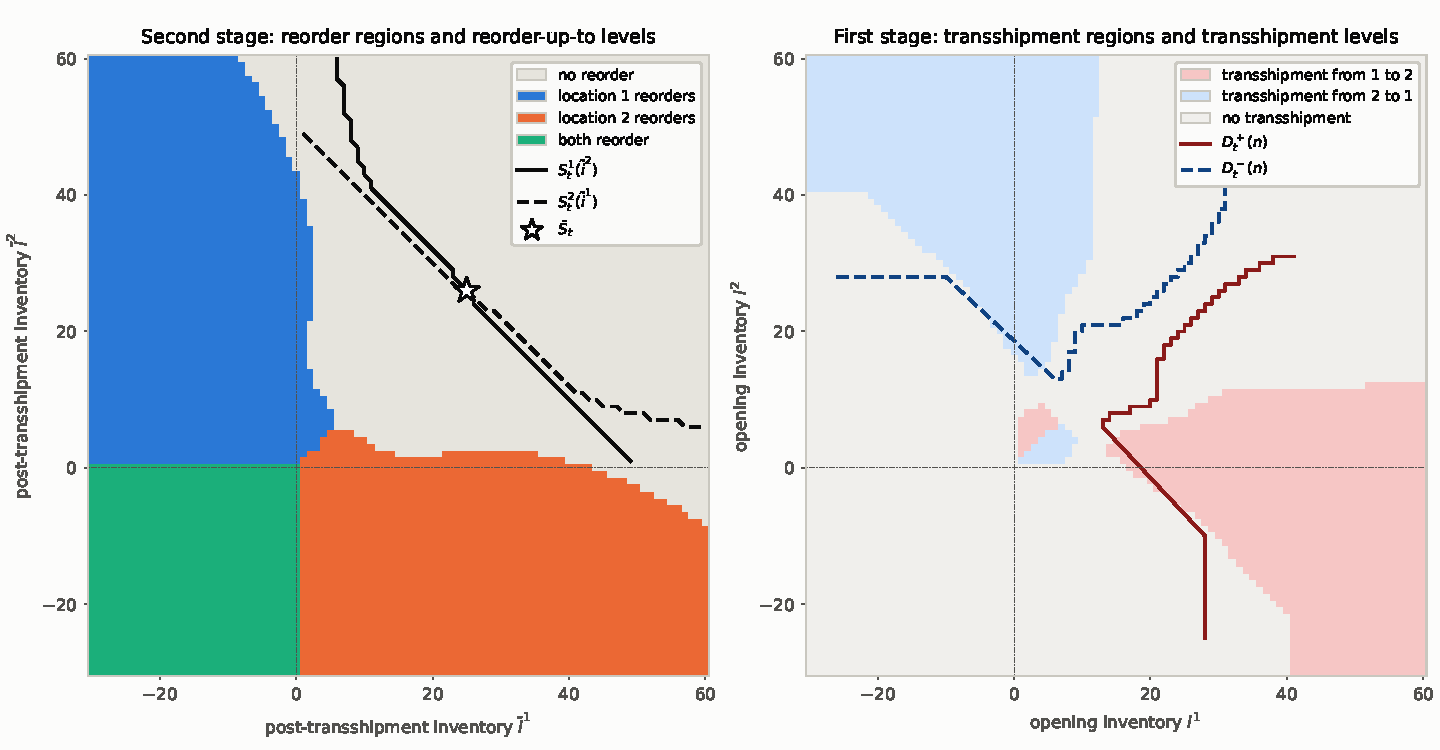
\includegraphics[width=\textwidth]{fig_levels_STAT-STAT_T4_K50_R2.pdf}
\caption{Levels of Theorem~\ref{thm:structure} in period~1 for the pair STAT--STAT with $T=4$, Poisson demand, $K=50$, $R=2$, $z=1$, $v=0.5$, $h=1$ and $b=5$. A level is drawn where the optimal policy uses it.}
\label{fig:levels}
\end{figure}

The theorem does not say that the region in which a location reorders is bounded by a threshold, and it does not say that the states without transshipment form an interval of each line. Both properties fail in general, as Sections~\ref{sec:threshold} and \ref{sec:false} show.

\section{Thresholds}\label{sec:threshold}

In a single-location problem the reorder region is $\{x\le s\}$. The corresponding statement here is that location~1 reorders at $\langle x^1,x^2\rangle$ if and only if $x^1\le s^1_t(x^2)$. By Lemma~\ref{lem:reduction} this is a property of the one-dimensional function $g^1_t(\cdot\,;x^2)$. This section gives a sufficient condition and then proves that the property fails in general.

\subsection{A sufficient condition}

\begin{proposition}[Sufficient condition]\label{prop:Q}
Fix $t$ and $x^2$ and write $g=g^1_t(\cdot\,;x^2)$. Suppose that
\begin{equation}\label{eq:Q}\tag{Q}
g(x)\le\max\{g(x'),\ K+g(y)\}\qquad\text{for all integers }x'<x<y .
\end{equation}
Then there is an integer $s^1_t(x^2)$ such that location~1 reorders in every optimal decision at $\langle x^1,x^2\rangle$ if and only if $x^1\le s^1_t(x^2)$. Condition~\eqref{eq:Q} holds if $g$ is $K$-convex.
\end{proposition}

\begin{proof}
Let $A$ be the set of $x$ that satisfy \eqref{eq:reorder1}, that is $g(x)>K+\min_{y>x}g(y)$. Let $x\in A$ and $x'<x$, and let $y^*>x$ attain the minimum. Then $g(x)>K+g(y^*)$, and \eqref{eq:Q} with the triple $x'<x<y^*$ gives $g(x)\le g(x')$. So $g(x')\ge g(x)>K+g(y^*)\ge K+\min_{y>x'}g(y)$ and $x'\in A$. The set $A$ is non-empty: $g(x)\ge\psi^1_t(x)+\min\psi^2_t\to\infty$ as $x\to-\infty$, whereas $K+\min_{y>x}g(y)$ does not increase as $x$ decreases. The set $A$ is bounded above: otherwise $A=\Z$, and starting from any point one finds $y_1<y_2<\cdots$ with $g(y_{k+1})<g(y_k)-K$, which contradicts that $g$ is bounded below. So $A=\{x\le s\}$ with $s=\max A$.

Let $g$ be $K$-convex on $\Z$, so that $K+g(y)\ge g(x)+\frac{y-x}{x-x'}\,(g(x)-g(x'))$ for all integers $x'<x<y$. If $g(x)>g(x')$, the last term is positive and $g(x)<K+g(y)$. Otherwise $g(x)\le g(x')$. In both cases \eqref{eq:Q} holds.
\end{proof}

Condition~\eqref{eq:Q} only forbids a point whose cost exceeds the cost of a lower point and also exceeds the cost of a higher point by more than $K$. In the last period $g^j_T$ equals the convex function $f^j$ of Lemma~\ref{lem:last} plus a constant, and \eqref{eq:Q} holds. In the earlier periods \eqref{eq:Q} can fail, and so can the threshold property.

\subsection{The threshold property can fail}

\begin{proposition}[No threshold in general]\label{prop:threshold}
There are instances that satisfy Assumptions~\ref{ass:demand} and \ref{ass:cost} in which a location reorders in every optimal decision at some inventory and in no optimal decision at a lower inventory, the inventory of the other location being the same. This happens in the following two instances with $T=2$, $R=2$, $z=1$, $v=\tfrac12$, $h=1$ and $b=20$. In both, the demands of periods~1 and 2 have the means $(1,30)$ at location~1 and $(1,12)$ at location~2.
\begin{enumerate}[label=(\alph*)]
\item \emph{Deterministic demand, $K=44.5$.} In period~1 and at the post-transshipment states $\langle x^1,3\rangle$, location~1 reorders in every optimal decision for $-2\le x^1\le0$ and for $4\le x^1\le9$. It reorders in no optimal decision for $1\le x^1\le3$ and for $10\le x^1\le13$. No transshipment is the only optimal first-stage decision at the opening states $\langle i^1,3\rangle$ with $1\le i^1\le9$.
\item \emph{Truncated Poisson demand, $K=57$.} Each demand has the Poisson distribution with its mean, restricted to the values $0,\ldots,6$ for the mean 1, $0,\ldots,52$ for the mean 30 and $0,\ldots,27$ for the mean 12, and renormalised. In period~1 and at the states $\langle x^1,3\rangle$, location~1 reorders in every optimal decision for $0\le x^1\le2$ and for $4\le x^1\le7$. It reorders in no optimal decision for $x^1=3$ and for $8\le x^1\le10$. No transshipment is the only optimal first-stage decision at the opening states $\langle i^1,3\rangle$ with $-1\le i^1\le11$.
\end{enumerate}
In both instances the states at which the threshold fails are opening states at which the optimal policy does not transship. They are therefore reached by every optimal policy that starts in them.
\end{proposition}

\begin{proof}
Both instances have two periods and demands with finitely many values and rational probabilities. The probabilities of the truncated Poisson distribution are $(\lambda^k/k!)/\sum_{i\le m}\lambda^i/i!$, and they are rational for an integer mean $\lambda$. The recursion can therefore be evaluated in exact rational arithmetic, and every comparison below is exact. The evaluation has three parts.

\emph{Period~2.} Lemma~\ref{lem:last} gives the second stage in closed form. The first stage is a minimum over the finite set $\R(\vec{i})$.

\emph{Second stage of period~1.} At a post-transshipment state $\vec{x}$ we enumerate the levels $\vec{y}\ge\vec{x}$ with $y^1\le100$ and $y^2\le100$. A level above 100 cannot be optimal. Indeed, \eqref{eq:ellbound} gives $\ell^j_1(y)\ge h(y-\mu^j_1)$. The bound $\Cq_2(\vec{x})\ge\theta^1_2(x^1)+\theta^2_2(x^2)\ge h(x^1+x^2-\mu^1_2-\mu^2_2)$ from the proof of Lemma~\ref{lem:line} carries over to $\Ct_2$, because a transshipment keeps the total inventory and its cost is non-negative. Let $M=44$ be the sum of the four expected demands. A decision with $y^j\ge101$ at the state $\vec{x}$ therefore costs at least
\[
z(101-x^j)+h(101-\mu^j_1)+h(101+x^k-M),\qquad k\ne j .
\]
At every state that we evaluate this bound exceeds the cost of the best decision found, by at least $111.5$ in instance (a) and by at least $49.16$ in instance (b).

\emph{First stage of period~1.} This is again a minimum over a finite set.

Tables~\ref{tab:det} and \ref{tab:threshold} report the cost of the best decision without a reorder at location~1 and the cost of the best decision with one, as defined in Lemma~\ref{lem:reduction}. Location~1 reorders in every optimal decision when the difference is positive and in no optimal decision when it is negative. In instance (a) the values not shown are $194$ and $173$ without a reorder at $x^1=-2,-1$, against $136.5$ and $135.5$ with one, and $93.5$ without a reorder at $x^1=12,13$, against $122.5$ and $121.5$. The script \texttt{exact\_examples.py} carries out the computation and uses no floating-point number.
\end{proof}

\begin{table}[h]
\centering
\footnotesize
\setlength{\tabcolsep}{3.2pt}
\caption{Instance (a) of Proposition~\ref{prop:threshold}: exact cost of the best reorder decision at $\langle x^1,3\rangle$ in period~1 without and with a reorder at location~1.}\label{tab:det}
\begin{tabular}{lrrrrrrrrrrrr}
\toprule
$x^1$ & 0 & 1 & 2 & 3 & 4 & 5 & 6 & 7 & 8 & 9 & 10 & 11 \\
\midrule
Without & 152 & 131 & 131 & 131 & 131 & 131 & 131 & 131 & 131 & 130.5 & 112 & 93.5 \\
With & 134.5 & 133.5 & 132.5 & 131.5 & 130.5 & 129.5 & 128.5 & 127.5 & 126.5 & 125.5 & 124.5 & 123.5 \\
Difference & 17.5 & $-2.5$ & $-1.5$ & $-0.5$ & 0.5 & 1.5 & 2.5 & 3.5 & 4.5 & 5 & $-12.5$ & $-30$ \\
Reorder at 1 & yes & no & no & no & yes & yes & yes & yes & yes & yes & no & no \\
\bottomrule
\end{tabular}
\end{table}

\begin{table}[h]
\centering
\footnotesize
\setlength{\tabcolsep}{2.0pt}
\caption{Instance (b) of Proposition~\ref{prop:threshold}: cost of the best reorder decision at $\langle x^1,3\rangle$ in period~1 without and with a reorder at location~1. The values are exact rational numbers, shown to four decimals.}\label{tab:threshold}
\begin{tabular}{lrrrrrrrrrr}
\toprule
$x^1$ & 0 & 1 & 2 & 3 & 4 & 5 & 6 & 7 & 8 & 9 \\
\midrule
Without & 210.6769 & 197.4030 & 191.8553 & 190.1705 & 189.7735 & 189.6984 & 189.5108 & 187.4096 & 182.0439 & 174.0828 \\
With & 193.6524 & 192.6524 & 191.6524 & 190.6524 & 189.6524 & 188.6524 & 187.6524 & 186.6524 & 185.6524 & 184.6524 \\
Difference & 17.0245 & 4.7506 & 0.2028 & $-0.4819$ & 0.1211 & 1.0460 & 1.8583 & 0.7571 & $-3.6085$ & $-10.5696$ \\
Reorder at 1 & yes & yes & yes & no & yes & yes & yes & yes & no & no \\
\bottomrule
\end{tabular}
\end{table}

\begin{illustration}[A tie]\label{ex:tie}
Take instance (a) with $K=45$ in place of $44.5$. The same exact computation gives the following for the state $\langle3,3\rangle$ in period~1. The best decision without a reorder at location~1 reorders nothing and costs 132. The best decision with a reorder at location~1 reorders 38 units there and also costs 132. No transshipment is the only optimal first-stage decision at the opening state $\langle3,3\rangle$. The actions $(0,0,0)$ and $(0,38,0)$ are therefore both optimal in this state. This is the example used in Proposition~\ref{prop:unique}.
\end{illustration}

\subsection{The mechanism}

Instance (a) can be followed by hand. Let $1\le x^1\le8$. Suppose first that location~1 does not reorder in period~1. The best decision then reorders nothing. The holding cost of period~1 is $h(x^1-1)+2h$, and period~2 opens in the state $\langle x^1-1,2\rangle$. There both locations reorder, up to 30 and 12, at the cost $2K+z(31-x^1)+10z=130-x^1$. The total is 131 for every such $x^1$. Suppose next that location~1 reorders up to 41 in period~1. This costs $K+z(41-x^1)$, and the holding cost of period~1 is $40h+2h$. Period~2 opens in the state $\langle40,2\rangle$. Location~1 ships 10 units to location~2 at the cost $R+10v=7$, and neither location reorders. The total is $134.5-x^1$. The reorder is the cheaper alternative if and only if $x^1>3.5$.

The reorder of period~1 is a reorder of location~1 for both locations. It saves the fixed reorder cost of location~2 in period~2 at the price of a transshipment and of one period of holding. One more unit on hand lowers the cost with this reorder by the unit cost $z$, because one unit less is bought. Without the reorder the additional unit is held for one period, and one unit less is bought in period~2. The cost then changes by $h-z$, and this is zero here. The reorder therefore becomes cheaper as the inventory rises, and the threshold is lost. At $x^1\le0$ location~1 reorders for another reason: it would otherwise backorder demand of period~1 at the cost $b$. At $x^1\ge10$ it does not reorder, because the stock that it already holds is enough to supply location~2 in period~2. In the state $\langle9,2\rangle$ of period~2, for example, location~1 ships its 9 units and then reorders alone. In terms of Lemma~\ref{lem:reduction}, $g^1_1(y;3)=134+y$ for $1\le y\le8$ and $g^1_1(41;3)=93$, so $g^1_1(4;3)=138$ exceeds both $g^1_1(1;3)=135$ and $K+g^1_1(41;3)=137.5$, and condition~\eqref{eq:Q} fails.

Instance (b) shows the same mechanism under Poisson demand. If neither location reorders in period~1, both reorder in period~2, for example in the state $\langle2,2\rangle$. If location~1 reorders up to 50 in period~1, it supplies location~2 in period~2. In the state $\langle50,2\rangle$ of period~2, for example, it ships 14 units and neither location reorders. At $\langle3,3\rangle$ the two alternatives are close, and waiting is cheaper by $0.4819$. With one more unit at location~1 the cost with the reorder falls by $z=1$. The cost without the reorder falls by less, by $0.3970$, $0.0751$ and $0.1876$ from 3 to 6 units. The reorder is therefore the cheaper alternative from 4 to 7 units.

The counterexample combines three ingredients. A reorder of one location for both must pay, so $K$ must exceed the cost $R+v|W|$ of the later transshipment plus the holding cost. The other location must not be able to take this role at the same cost, which holds here because the demand of location~1 in period~2 is larger. The fixed reorder cost must lie in the range in which the two alternatives are close. For instance (a) this range is $39.5\le K\le46.5$ in steps of $0.5$, by the same exact computation. A targeted search of Section~\ref{sec:numerics} finds the same failure for normal demand with $\rho=0.1$, $0.2$ and $0.3$. Section~\ref{sec:stress} reports what happens when $K\le R+v$.

The thresholds, where they exist, are not monotone in general: in the pair STAT--STAT with $T=4$, $K=50$ and $R=2$ the threshold of location~1 in period~1 takes the values $1,5,4,2,1,2$ at $\tilde{i}^2=2,6,10,14,18,22$.

\section{Further properties that do not hold}\label{sec:false}

The results for unit costs suggest two further properties: the states without transshipment form an interval of every line of constant total inventory, and the value function has a convexity property that the recursion preserves. Both fail, and they fail already in a problem with one period.

\begin{proposition}[One period]\label{prop:oneperiod}
Let $T=1$, let the demand be 3 at each location with probability one, and let $K=20$, $R=2$, $z=1$, $v=\tfrac12$, $h=1$ and $b=20$. Assumptions~\ref{ass:demand} and \ref{ass:cost} hold, and the following is true.
\begin{enumerate}[label=(\roman*)]
\item On the line $i^1+i^2=3$ a transshipment is made in every optimal action at $i^1=-2$, in no optimal action at $i^1=-1$ and $i^1=0$, in every optimal action at $i^1=1$ and $i^1=2$, in no optimal action at $i^1=3$ and $i^1=4$, and in every optimal action at $i^1=5$. The states without transshipment are not an interval of the line.
\item At $\langle1,2\rangle$ location~1 ships its unit to location~2, and at $\langle2,1\rangle$ location~2 ships its unit to location~1. The sender is the location with less stock.
\item $\Ct_1$ is not $K$-convex in $i^1$: $K+\Ct_1(6,0)-\Ct_1(0,0)<6\,\big(\Ct_1(0,0)-\Ct_1(-1,0)\big)$.
\end{enumerate}
\end{proposition}

\begin{proof}
By Lemma~\ref{lem:last}, $f^j(y)=zy+h\max\{0,y-3\}+b\max\{0,3-y\}$, $S^j_1=3$, and location $j$ reorders if and only if $19\,(3-x)>20$, that is $x\le1$. The second-stage cost of one location is therefore $c(x)=K+z(3-x)=23-x$ for $x\le1$, $c(2)=b=20$ and $c(x)=h(x-3)$ for $x\ge3$. On the line $i^1+i^2=3$ the second-stage value is $G(x)=c(x)+c(3-x)$, with
\begin{align*}
G(-2)&=27, & G(-1)&=25, & G(0)&=23, & G(1)&=42,\\
G(2)&=42, & G(3)&=23, & G(4)&=25, & G(5)&=27 .
\end{align*}
A transshipment from the state with $i^1$ to the post-transshipment state with $x$ costs $2+\tfrac12|i^1-x|$. It is feasible for $0\le x<i^1$ and for $i^1<x\le3$.

(i) At $i^1=-2$ the targets $x=-1,0,1,2,3$ cost $27.5$, $26$, $45.5$, $46$ and $27.5$, and no transshipment costs 27, so the transshipment to $x=0$ is the only optimal decision. At $i^1=-1$ the best target is $x=0$ at $25.5$, against 25 without transshipment. At $i^1=0$ the best target is $x=3$ at $26.5$, against 23. At $i^1=1$ the targets $x=0,2,3$ cost $25.5$, $44.5$ and $26$, against 42. At $i^1=2$ the targets $x=0,1,3$ cost $26$, $44.5$ and $25.5$, against 42. At $i^1=3$ the best target is $x=0$ at $26.5$, against 23. At $i^1=4$ the best target is $x=3$ at $25.5$, against 25. At $i^1=5$ the target $x=3$ costs 26, against 27.

(ii) This was shown in (i): the only optimal target is $x=0$ at $i^1=1$ and $x=3$ at $i^1=2$.

(iii) No transshipment is feasible at $\langle0,0\rangle$ and at $\langle-1,0\rangle$, so $\Ct_1(0,0)=2c(0)=46$ and $\Ct_1(-1,0)=c(-1)+c(0)=47$. At $\langle6,0\rangle$ a transshipment of 3 units costs $3.5$ and leaves no further cost, so $\Ct_1(6,0)\le3.5$. Hence $K+\Ct_1(6,0)-\Ct_1(0,0)\le-22.5<-6$.
\end{proof}

The cause of (i) is the kink of the second-stage cost at the reorder threshold. A location at or below the threshold reorders in any case, so stock that is shipped to it saves only the unit cost. A location just above the threshold does not reorder and is short, so stock that is shipped to it saves the backorder cost. The cause of (iii) is that stock at location~1 can serve location~2 through a transshipment, so it saves more than one fixed reorder cost. The minimisation over the transshipment in \eqref{eq:first} does not preserve $K$-convexity, and the classical proof of the $(s,S)$ policy does not extend.

The two-period instance (a) of Proposition~\ref{prop:threshold} gives a third exact statement. The level $S^1_1(x^2)$ of Theorem~\ref{thm:structure} is the only minimiser of $H_1(\cdot,x^2)$ and equals $44-x^2$ for $2\le x^2\le12$, by the computation of that proposition. The reorder-up-to level of location~1 therefore depends on the inventory of location~2. Location~1 reorders for the needs of both locations and raises the total stock to 44, the total demand of the two periods.

The same properties fail in instances with Poisson demand and four periods. The following observations are computed with SDP-2 in double precision on a range of inventory levels that is wide enough for no demand outcome to be dropped on the states shown. All instances have $T=4$, Poisson demand, $z=1$, $v=0.5$, $h=1$ and $b=5$. The expected demands are $(7,7,7,7)$ for STAT, $(2,5,10,11)$ for LCY1, $(6,13,7,2)$ for LCY2 and $(2,2,2,2)$ for STAT/3. Every difference quoted is larger than $10^{-2}$, far above rounding.

\begin{example}[The states without transshipment are not an interval of a line]\label{ex:interval}
STAT--STAT, $K=50$, $R=2$, period~1, line $n=10$. No transshipment is made at $\langle1,9\rangle$. At $\langle2,8\rangle$, $\langle3,7\rangle$ and $\langle4,6\rangle$ location~1 ships all its stock to location~2 and then reorders. At $\langle5,5\rangle$ to $\langle8,2\rangle$ location~2 ships all its stock to location~1 and then reorders. No transshipment is made at $\langle9,1\rangle$. At $\langle2,8\rangle$ the optimal action is $(W,Q^1,Q^2)=(2,40,0)$ with $\Ct_1=211.395$, against $\Cq_1=212.037$ without transshipment.
\end{example}

\begin{example}[The same failure in the last period]\label{ex:last}
LCY1--LCY2, $K=50$, $R=2$, period~4, line $n=-1$. No transshipment is made at $\langle9,-10\rangle$. At $\langle10,-11\rangle$ and $\langle11,-12\rangle$ location~1 ships 3 and 4 units. At $\langle12,-13\rangle$ to $\langle15,-16\rangle$ no transshipment is made and location~2 reorders. At $\langle16,-17\rangle$ location~1 ships 9 units. Every transshipment ends at $\tilde{\vec{i}}=\langle7,-8\rangle$, which is the level $D^+_4(-1)=7$ of Theorem~\ref{thm:structure}.
\end{example}

\begin{example}[$\Ct_t$ is not $K$-convex]\label{ex:kconv}
STAT--STAT, $K=50$, $R=2$, period~1. $\Ct_1(-1,0)=259.549$, $\Ct_1(0,0)=258.549$ and $\Ct_1(50,0)=122.585$. $K$-convexity in $i^1$ requires $\Ct_1(50,0)+K\ge\Ct_1(0,0)+50\,(\Ct_1(0,0)-\Ct_1(-1,0))=208.549$, but the left-hand side is $172.585$.
\end{example}

\begin{example}[$\Cq_t$ is not $K$-convex when $K=R$]\label{ex:kconv2}
STAT--STAT/3, $K=20$, $R=20$, period~1. $\Cq_1(4,11)=116.090$, $\Cq_1(4,12)=119.079$ and $\Cq_1(4,38)=136.713$. $K$-convexity in $\tilde{i}^2$ requires $\Cq_1(4,38)+K\ge\Cq_1(4,12)+26\,(\Cq_1(4,12)-\Cq_1(4,11))=196.800$, but the left-hand side is $156.713$.
\end{example}

\begin{example}[The reorder-up-to level of one location depends on the other]\label{ex:slope}
STAT--STAT, $K=50$, $R=2$, period~1. $S^1_1(\tilde{i}^2)=48,44,40,36,32,28$ at $\tilde{i}^2=2,6,10,14,18,22$, so $S^1_1(\tilde{i}^2)+\tilde{i}^2=50$. The single-location level is 25. The location that reorders raises the total stock of the two locations to twice the single-location level and transships later. With $K=20$ and $R=20$ the level is 21 for $\tilde{i}^2=5,9,\ldots,29$, which is the single-location level.
\end{example}

\section{Numerical tests}\label{sec:numerics}

\subsection{Instances and method}

We test four sets of instances, 336 in total, all with $h=1$.
\begin{itemize}
\item Set A is test bed~II of the companion paper at $T=4$: $K\in\{20,30,50\}$, $R\in\{2,5,10,20\}$, Poisson demand and normal demand with $\rho\in\{0.1,0.3\}$, six relations between the demand patterns, $z=1$, $v=0.5$ and $b=5$; 216 instances.
\item Set B is test bed~II at $T=8$ with $(K,R)\in\{(20,20),(20,2),(50,20),(50,2)\}$, Poisson demand and normal demand with $\rho=0.3$, and the six relations; 48 instances.
\item Set C uses $b=3$, $z=2$ and $v=1$ at $T=4$ with $K\in\{10,30\}$, $R\in\{5,20\}$, Poisson demand and normal demand with $\rho=0.2$, and the pairs STAT--STAT, LCY1--LCY2, STAT--STAT/3 and RAND--EMP1; 32 instances.
\item Set D lies outside the test beds of the companion paper. It uses five cost settings at $T=4$, namely $(K,R,z,v,b)=(100,2,1,0.5,5)$, $(5,20,1,0.5,5)$, $(20,5,1,1,10)$, $(30,10,2,0.5,3)$ and $(50,50,1,0.5,20)$, with Poisson demand and normal demand with $\rho=0.3$, and the pairs SIN1--SIN2, RAND--RAND, EMP1--EMP2 and LCY2--SIN1; 40 instances.
\end{itemize}
Every instance satisfies Assumptions~\ref{ass:demand} and \ref{ass:cost}. SDP-2 is solved with the code of the companion paper on the range of inventory levels $[lo-TD,\ hi]$, where $[lo,hi]$ is the adequate range of the companion paper and $D$ is the largest truncated demand of a period. On this range no demand outcome is dropped for the states of the window $[lo,hi]^2$. All tests are run on every state of the window in every period, which gives 1,536 instance-periods and 9,260,688 states. An action is called strictly optimal when the best alternative is worse by more than $10^{-8}$. The levels $\bar{\vec{S}}_t$, $S^j_t$, $D^+_t$ and $D^-_t$ are computed from $H_t$ and $\Cq_t$ as in Section~\ref{sec:lemmas} and are then compared with the policy returned by SDP-2.

\subsection{Checks of the proved statements}

The proved statements need no numerical confirmation. The checks guard against an error in a proof or in the code. Table~\ref{tab:checks} counts the states that contradict each statement.

\begin{table}[h]
\centering
\small
\setlength{\tabcolsep}{4pt}
\caption{Number of states that contradict a statement of Theorem~\ref{thm:structure}, and number of rows of the state space that contradict the threshold property or condition \eqref{eq:Q}.}\label{tab:checks}
\begin{tabular}{lrrrrrrrrr}
\toprule
 & & & & \multicolumn{4}{c}{Theorem~\ref{thm:structure}} & \multicolumn{2}{c}{Thresholds} \\
\cmidrule(lr){5-8}\cmidrule(lr){9-10}
Set & Instances & States & Transshipments & (a) & (b) & (c) & (d) & Threshold & \eqref{eq:Q} \\
\midrule
A & 216 & 4,683,312 & 1,591,935 & 0 & 0 & 0 & 0 & 0 & 0 \\
B & 48 & 2,745,992 & 901,471 & 0 & 0 & 0 & 0 & 0 & 0 \\
C & 32 & 720,188 & 239,606 & 0 & 0 & 0 & 0 & 0 & 0 \\
D & 40 & 1,111,196 & 371,516 & 0 & 0 & 0 & 0 & 0 & 0 \\
\midrule
All & 336 & 9,260,688 & 3,104,528 & 0 & 0 & 0 & 0 & 0 & 0 \\
\bottomrule
\end{tabular}
\end{table}

\emph{Part (a).} A transshipment is strictly optimal in 3,104,528 opening states. Of these, 3,045,814 states, or 98.1\%, lie beyond the transshipment level of their line, and every one of them reaches the level $D^+_t(n)$ or $D^-_t(n)$ in value. The other 1.9\% ship to a constrained target as described after Lemma~\ref{lem:line}. No state beyond a level stays without transshipment although the level is cheaper by more than $R$, and $D^-_t(n)\le D^+_t(n)$ on every line. The largest number of distinct targets on one line and in one direction is 3.

\emph{Part (b).} A reorder is made in 5,073,291 post-transshipment states. Every one of them lies below the level of its pattern and reaches it in value: $\bar{\vec{S}}_t$ when both locations reorder and $S^j_t$ when location $j$ reorders alone. The point $\bar{\vec{S}}_t$ and the two curves therefore describe all reorders of the optimal policy in the tested instances.

\emph{Part (c).} No transshipment is followed by reorders at both locations. The sender reorders after the transshipment in 41,631 states, always more than $|W|$ units and always with $K\ge R+v|W|$. In the 54 instances with $K<R+v$ a transshipment is made in 353,505 states and the sender never reorders. The receiver reorders after the transshipment in 283,630 states.

\emph{Part (d).} In the last period the thresholds and the levels of both locations are the same for every inventory of the other location and equal the single-location values $(s^j_T,S^j_T)$. In 24 of the 672 cases the threshold $s^j_T$ lies below the window, and the location does not reorder at any state of the window, as the lemma requires.

\subsection{Threshold property on the 336 instances}

Condition~\eqref{eq:Q} holds for $g^1_t$ and $g^2_t$ at every inventory of the other location in all 1,536 instance-periods, and each location reorders exactly at or below a threshold of its own inventory. Of these instance-periods 1,200 lie before the last period, with 7,288,765 states, and there the property is not covered by a proof. In the instances that follow the test beds of the companion paper the optimal reorder decision is therefore of threshold type, although Proposition~\ref{prop:threshold} shows that this is not true in general.

\subsection{Targeted search for a failure of the threshold property}

The mechanism of Section~\ref{sec:threshold} suggests where to look. We test 543 two-period instances with $R=2$ unless stated, $z=1$, $v=0.5$, $h=1$ and $b=20$, in four families.
\begin{itemize}
\item Expected demands $(7,20)$ and $(7,3)$, $K$ from 20 to 32 in steps of 0.25, Poisson demand and normal demand with $\rho\in\{0.01,0.03,0.05,0.1,0.2,0.3\}$; 343 instances. The threshold property fails in period~1 for $\rho=0.01$ at $K$ from 25.75 to 26.25 and for $\rho=0.03$ at $K$ from 26.75 to 27.25. It holds for the other demand models in this range of $K$.
\item Expected demands $(1,30)$ and $(1,12)$, $K$ from 36 to 54 in steps of 1, Poisson demand and normal demand with $\rho\in\{0.1,0.2,0.3\}$; 76 instances. The property fails for $\rho=0.1$ at $K$ from 43 to 54, for $\rho=0.2$ at $K$ from 49 to 54 and for Poisson demand at $K=54$.
\item The same demands with $K$ from 55 to 80, Poisson demand and normal demand with $\rho=0.3$; 52 instances. The property fails for Poisson demand at $K$ from 55 to 60 and for $\rho=0.3$ at $K$ from 56 to 65. Condition~\eqref{eq:Q} fails on a wider range, up to $K=66$ and $K=75$.
\item Both pairs of demands with $K\in\{20,30,40,50,57,60\}$ and $R\in\{K-0.5,\,K,\,K+10\}$, so that $K\le R+v$; 72 instances. The property and condition~\eqref{eq:Q} hold in every instance.
\end{itemize}
Every failure occurs in period~1 and at location~1, the location with the larger demand in period~2. No failure occurs in period~2, in agreement with Lemma~\ref{lem:last}. The failure also occurs when only the post-transshipment states reached by the optimal policy are considered.

\subsection{Stress test on extreme instances}\label{sec:stress}

The instances above have moderate parameters. A further test uses extreme ones. Its purpose is twofold: to look for an instance that contradicts a proved statement, and to look for regularities of the optimal policy that the theorem does not contain. All instances have $z=1$.
\begin{itemize}
\item \emph{Corners.} Every combination of $K\in\{0.5,300\}$, $R\in\{0.1,300\}$, $v\in\{0.01,1\}$, $b\in\{1.05,100\}$ and $h\in\{0.05,10\}$, with Poisson demand, $T=3$ and three pairs of demand patterns: $(6,6,6)$ at both locations, $(1,1,1)$ against $(14,14,14)$, and $(1,1,18)$ against $(1,18,1)$; 96 instances.
\item \emph{Random.} The costs are drawn independently with a uniform distribution of their logarithm, $K\in[0.5,300]$, $R\in[0.1,300]$, $v\in[0.01,1]$, $b\in[1.05,100]$ and $h\in[0.05,10]$. The horizon is drawn from 2 to 5 periods. The demand is Poisson or normal with $\rho\in\{0.02,0.1,0.3,0.5\}$. The pair of demand patterns is drawn from ten pairs. They include equal, very unequal, increasing against decreasing, alternating and peaked demands and a location with almost no demand. The expected demands are scaled down where needed so that an instance can be solved in a few minutes; 600 instances, of which 599 could be solved. For one instance the search for an adequate range of inventory levels did not end within its limit. For six instances a reorder-up-to level of a state of the window lay above the adequate range, and they were solved again on a wider range.
\end{itemize}
The 695 solved instances have 2,365 instance-periods and 17,533,871 states of the window, and 303 of them have $K\le R+v$. A fixed cost of $0.5$ against a unit cost of 1 makes the fixed costs almost irrelevant, and a fixed cost of 300 exceeds the unit cost of the whole demand of the horizon. A backorder cost of $1.05$ is just above the unit cost, so backordering is almost free.

\emph{Proved statements.} No state contradicts Theorem~\ref{thm:structure}. The counts that correspond to Table~\ref{tab:checks} are all zero. A transshipment is strictly optimal in 6,192,213 opening states, and 6,110,776 of them lie beyond the transshipment level of their line and reach it in value. A reorder is made in 7,483,074 post-transshipment states, and 7,470,374 of them lie below the level of their pattern and reach it in value. In the moderate instances every reorder was of this kind. In the extreme instances 12,700 reorders start at or above the level and go to a constrained minimiser, as Lemma~\ref{lem:patterns} allows. The sender reorders after a transshipment in 76,291 states, always with $K\ge R+v|W|$, and never in the 303 instances with $K<R+v$. In the last period the thresholds and the levels agree with Lemma~\ref{lem:last} in all 1,390 cases.

\emph{Threshold property.} We test the property on two sets of states. The first is the set of all post-transshipment states of the window. The second is the set of \emph{reached} states. A post-transshipment state is reached if the computed optimal policy moves to it from some opening state of the window, and an opening state without transshipment is reached from itself.
At the set of all post-transshipment states the property fails in 20 of the 695 instances, in 31 instance-periods. Of these instances 18 have $K\le R+v$ and 2 have $K>R+v$. Condition~\eqref{eq:Q} fails in 26 instances. No failure occurs in the last period. At the reached states the property fails in 2 instances and holds in the other 693. Both have $K>R+v$ and normal demand with $\rho=0.02$. Both have the demand pattern of Proposition~\ref{prop:threshold}: the expected demand of location~1 alternates between 1 and a large value, and that of location~2 between 1 and a smaller value. They are further cases of the mechanism of Section~\ref{sec:threshold}. In the 303 instances with $K\le R+v$ the property holds at every reached state. In these tests the threshold property with $K\le R+v$ therefore fails only at states that the optimal policy does not reach.

\begin{remark}[A failure at states that are not reached]\label{obs:unreached}
The following instance has $K\le R+v$ and can be checked exactly. Let $T=2$, let the demand be 2 at each location in each period with probability one, and let $K=1$, $R=10$, $z=1$, $v=1$, $h=3$ and $b=2$. The exact computation of Proposition~\ref{prop:threshold} gives the following for period~1 and the post-transshipment states $\langle x^1,20\rangle$. The best decision without a reorder at location~1 costs 108 for $-12\le x^1\le1$. The best decision with a reorder at location~1 costs 110 for $-12\le x^1\le-2$, 109 for $x^1=-1$ and 107 for $x^1=1$. Location~1 therefore reorders in every optimal decision at $x^1=1$ and in no optimal decision at $-12\le x^1\le-1$. The reason is that location~2 holds a large surplus. A location with a large backlog waits for a transshipment of this surplus in period~2, and a location with a small need reorders at once because the fixed transshipment cost is too high for a small quantity. These states are not reached. At every opening state $\langle x^1,20\rangle$ with $-12\le x^1\le1$ the only optimal first-stage decision is a transshipment from location~2. It ships the surplus in period~1. No opening state on the same line within 40 units has an optimal transshipment that ends in one of these states. In this instance a transshipment that pays in period~2 pays even more in period~1. The first stage therefore removes the states at which the second stage would wait.
\end{remark}

\subsection{Further regularities}\label{sec:regular}

The results for unit costs contain monotonicity properties, and the test looks for their counterparts. Table~\ref{tab:regular} counts the exceptions over the 695 extreme instances. No property of the table holds in all instances.

\begin{table}[h]
\centering
\small
\caption{Properties that are not part of Theorem~\ref{thm:structure}, and the number of the 695 extreme instances in which each fails in at least one period.}\label{tab:regular}
\begin{tabular}{p{11.2cm}r}
\toprule
Property & Instances with a failure \\
\midrule
The reorder-up-to curve $S^j_t(x)$ does not increase in the inventory $x$ of the other location & 141 \\
The curve $S^j_t(x)$ falls by at most one unit per unit of $x$ & 226 \\
The transshipment levels $D^+_t(n)$ and $D^-_t(n)$ do not decrease in the total inventory $n$ & 433 \\
The levels rise by at most one unit per unit of $n$ & 453 \\
A sender that reorders after the transshipment ships all its stock & 261 \\
$\Cq_t$ is supermodular & 535 \\
$\Cq_t$ is submodular & 572 \\
The states without transshipment form an interval of every line & 331 \\
$\Ct_t$ is $K$-convex in each coordinate & 560 \\
$\Cq_t$ is $K$-convex in each coordinate & 312 \\
\bottomrule
\end{tabular}
\end{table}

Ties are never counted as failures. A curve or a level enters the count only where the optimal policy uses it and where its minimiser does not lie at an end of the window. The ten types of action that Corollary~\ref{cor:types} allows, with the direction of the transshipment counted separately, all occur: 197 instance-periods contain all ten, and each type occurs in at least 186 instances. The stress test therefore supports the view that Theorem~\ref{thm:structure} states what holds in general. The properties that the models with unit costs add to it are lost with the fixed costs.

\subsection{Frequency of the properties that fail}

Table~\ref{tab:fail} shows how often the properties of Section~\ref{sec:false} fail.

\begin{table}[h]
\centering
\small
\setlength{\tabcolsep}{5pt}
\caption{Instances in which a property fails in at least one period, and lines $i^1+i^2=n$ on which the states without transshipment are not an interval.}\label{tab:fail}
\begin{tabular}{lrrrrr}
\toprule
 & & \multicolumn{2}{c}{Interval of each line} & \multicolumn{2}{c}{$K$-convexity in a coordinate} \\
\cmidrule(lr){3-4}\cmidrule(lr){5-6}
Set & Instances & Instances & Lines (\%) & $\Ct_t$ & $\Cq_t$ \\
\midrule
A & 216 & 206 & 6.23 & 215 & 167 \\
B & 48 & 39 & 5.35 & 48 & 30 \\
C & 32 & 16 & 1.40 & 32 & 27 \\
D & 40 & 24 & 3.27 & 40 & 20 \\
\midrule
All & 336 & 285 & 5.26 & 335 & 244 \\
\bottomrule
\end{tabular}
\end{table}

The states without transshipment fail to be an interval on 11,872 of the 225,552 lines, in 285 instances. In test bed~II the share of these lines rises with the ratio of the fixed costs: 2.23\% for $K/R\le2$, 5.54\% for $2<K/R\le4$ and 7.70\% for $K/R\ge5$. $\Ct_t$ is not $K$-convex in a coordinate in 335 instances. The exception is STAT--STAT with normal demand, $\rho=0.1$, $K=20$ and $R=20$, in which a transshipment is made in 0, 0, 14 and 164 states of periods 1 to 4 and the two locations are almost independent. $\Cq_t$ is not $K$-convex in a coordinate in 244 instances. The threshold of at least one location increases somewhere in the inventory of the other location in 869 of the 1,200 instance-periods before the last period.

\subsection{Limits}

The 336 instances cover Poisson demand and normal demand, horizons of 4 and 8 periods and expected demands of about 7 units per period. The targeted search covers two periods and two pairs of demand patterns. The stress test covers horizons of 2 to 5 periods, and its expected demands are limited by the time that an exact solution takes. All tests work on a finite window of inventory levels. None of them delimits the set of instances in which the threshold property holds at the reached states.

\section{Summary and open questions}\label{sec:summary}

Table~\ref{tab:status} lists the status of each statement.

\begin{table}[h]
\centering
\small
\caption{Status of the statements.}\label{tab:status}
\begin{tabular}{p{9.3cm}l}
\toprule
Statement & Status \\
\midrule
An optimal policy exists and is deterministic and Markov & proved, Theorem~\ref{thm:existence} \\
A policy is optimal if and only if it chooses optimal actions & proved, Proposition~\ref{prop:unique} \\
The optimal value is unique & proved, Proposition~\ref{prop:unique} \\
The optimal policy is unique & false, Example~\ref{ex:tie} \\
Reorder-up-to point $\bar{\vec{S}}_t$ and curves $S^1_t$, $S^2_t$ & proved, Theorem~\ref{thm:structure}(b) \\
Transshipment levels $D^-_t(n)\le D^+_t(n)$ on every line & proved, Theorem~\ref{thm:structure}(a) \\
No transshipment followed by two reorders & proved, Theorem~\ref{thm:structure}(c) \\
The sender reorders only if $K\ge R+v|W|$ & proved, Theorem~\ref{thm:structure}(c) \\
Independent $(s,S)$ policies in the last period & proved, Theorem~\ref{thm:structure}(d) \\
Threshold in the own inventory under condition \eqref{eq:Q} & proved, Proposition~\ref{prop:Q} \\
Threshold in the own inventory for $t<T$ & false, Proposition~\ref{prop:threshold} \\
Threshold at the reached states when $K\le R+v$ & open, no failure found \\
Threshold at every post-transshipment state when $K\le R+v$ & false, Remark~\ref{obs:unreached} \\
Thresholds monotone in the other inventory & false, Section~\ref{sec:threshold} \\
Reorder-up-to level independent of the other location & false, Section~\ref{sec:false} \\
States without transshipment form an interval of each line & false, Proposition~\ref{prop:oneperiod} \\
$K$-convexity of $\Ct_t$ & false, Proposition~\ref{prop:oneperiod} \\
$K$-convexity of $\Cq_t$ for $t<T$ & false, Counterexample~\ref{ex:kconv2} \\
Monotone reorder-up-to curves and transshipment levels & false, Section~\ref{sec:numerics} \\
\bottomrule
\end{tabular}
\end{table}

The optimal policy of the two-location problem with fixed costs on both actions is described by five objects per period. They are the targets of the actions, and the fixed costs decide by a comparison of costs whether a target is used. This is what remains of the switching-curve policies of the models with unit costs. The regions of the actions are not bounded by thresholds or by monotone curves in general, and the paper shows by exact counterexamples that no description of this kind can hold for all instances.

Three questions are open. The first is a condition on the parameters under which each location reorders below a threshold at the states that the optimal policy reaches. The mechanism of Proposition~\ref{prop:threshold} needs $K>R+v$, and no failure at a reached state was found when $K\le R+v$. A proof would have to show that a weaker form of condition~\eqref{eq:Q} is preserved by the recursion in this case. The second is a description of the functions $\varphi^{+}_{t,n}$ and $\varphi^{-}_{t,n}$ that would replace the comparison with $R$ in Theorem~\ref{thm:structure}(a) by thresholds in the cases in which the states without transshipment form an interval. The third is the regime of a large ratio $K/R$, in which the levels satisfy $S^1_t(\tilde{i}^2)+\tilde{i}^2=\text{constant}$ over a wide range and the two locations behave like one location with pooled stock. A policy with few parameters that is built from the five objects, and its distance from the optimum, is a further topic.

\bibliographystyle{plainnat}
\bibliography{policy_structure}

\end{document}
